\begin{figure}
\centering
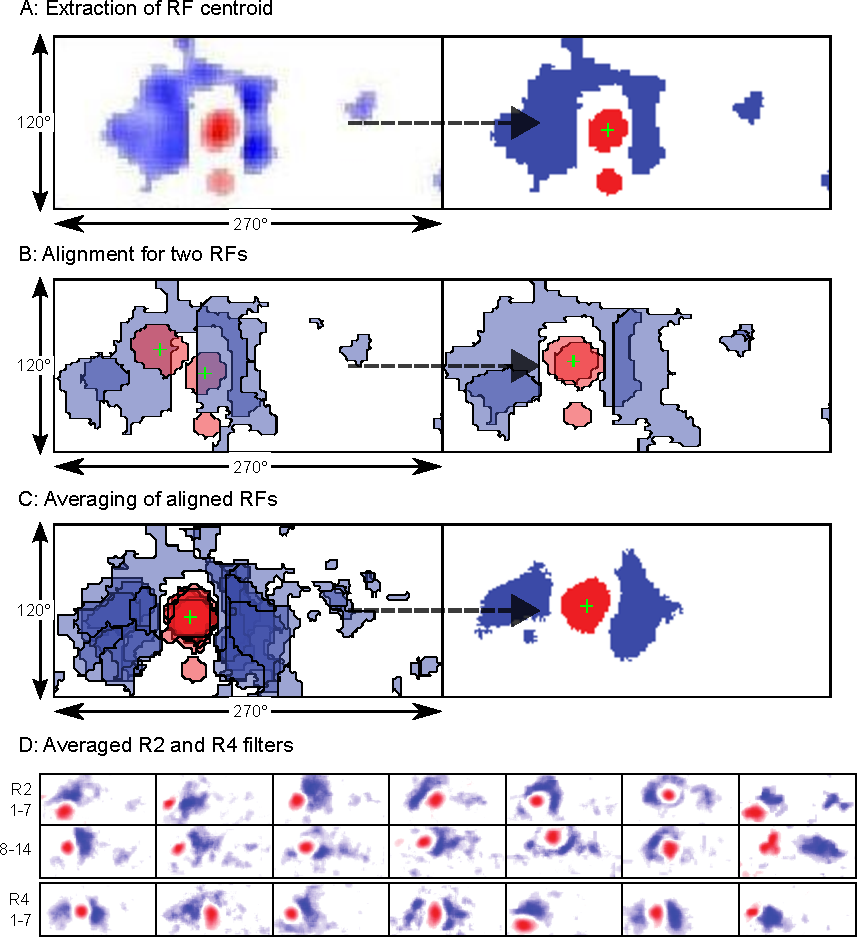
\includegraphics{figures/avkernels}
\caption{The algorithm for obtaining average RFs.
A: The raw image (left) is thresholded so as to give excitatory and inhibitory regions of uniform intensity (right).
The `centre' is then calculated as the centroid of the largest excitatory region (+).
B: Aligning two RFs.
The new centre is taken as the average of the centre of both RFs and the RFs are then shifted so that the centres are aligned.
C: Averaging the RFs for this glomerulus over all flies ($N=7$), following alignment.
Note that this the left-hemispheric version; the right-hemispheric version is its mirror.
Data are all for R4d glomerulus 1 neurons.}
\label{fig:avkernels}
\end{figure}
